\documentclass{article}

%% Language and font encodings
\usepackage[english]{babel}
\usepackage[utf8x]{inputenc}
\usepackage[T1]{fontenc}
\usepackage{verbatim} % multiline comments

%% Sets page size and margins
\usepackage[a4paper,top=3cm,bottom=2cm,left=3cm,right=3cm,marginparwidth=1.75cm]{geometry}

%% Useful packages
\usepackage{amsmath}
\usepackage{float}
\usepackage{rotating}
\usepackage{booktabs}
%\restylefloat{figure} % for force placing figures
%\floatplacement{figure}{H}
%\floatplacement{table}{H}
%\floatplacement{longtable}{H}
%\usepackage[markers,nolists]{endfloat}
\usepackage{graphicx}
\usepackage[colorinlistoftodos]{todonotes}
\usepackage[colorlinks=true, allcolors=blue]{hyperref}
%\usepackage{apalike}
\usepackage[round]{natbib}
\usepackage[switch]{lineno} % line numbers
\usepackage{longtable}
\usepackage{multirow}
% Supp mat
\newcommand{\beginsupplement}{%
        \setcounter{table}{0}
        \renewcommand{\thetable}{S\arabic{table}}%
        \setcounter{figure}{0}
        \renewcommand{\thefigure}{S\arabic{figure}}%
     }



\title{Dewlap color variation in \textit{Anolis sagrei} is maintained between habitats within islands of the West Indies}
\author{
    \textsc{Rapha\"{e}l Scherrer$^{1,3}$ \thanks{Corresponding author: r.scherrer@rug.nl}, Colin M. Donihue$^{1,4}$, }\\
	\textsc{R. Graham Reynolds$^2$, Jonathan B. Losos$^{1,4}$ and Anthony J. Geneva$^1$} \\[1ex]
	%\thanks{A thank you} \\[1ex] % Your name
	\normalsize $^1$ Department of Organismic and Evolutionary Biology and Museum of Comparative Zoology \\ \normalsize Harvard University, Cambridge, MA, USA \\
	\normalsize $^2$ Department of Biology, University of North Carolina Asheville, Asheville, NC, USA\\ % Your institutionhttps://www.overleaf.com/project/5a0705e5f4573c1ace38dbdf
	\normalsize $^3$ Current address: Groningen Institute for Evolutionary Life Sciences,\\
	\normalsize Groningen, The Netherlands\\
	\normalsize $^4$ Current address: Department of Biology, Washington University, St. Louis, MO, USA\\
}
\date{} % Leave empty to omit a date



\begin{document}
	
\linenumbers
	
\maketitle

\begin{abstract}
    Animal signals evolve in an ecological context. Moreover, locally adapting animal sexual signals can be especially important for initiating or reinforcing reproductive isolation during the early stages of speciation. Dewlap color in \textit{Anolis} lizards can be highly variable between populations in relation to both biotic and abiotic adaptive drivers, albeit at relatively large geographical scales. Here, we investigated local adaptation of the dewlap across habitat-types at a small spatial scale, as this may give an indication of how conditions for the early stages of speciation may be met. We explored variation in dewlap coloration in the most widespread species of anole, \textit{Anolis sagrei}, across three characteristic habitats spanning the Bahamas and the Cayman Islands. Using reflectance spectrometry as well as supervised machine learning, we found some consistent differences in spectral properties of the dewlap between habitats within small islands. Passive divergence in dewlap phenotype associated with isolation-by-distance did not explain our results. Instead, the observed patterns in dewlap coloration are more consistent with an adaptive explanation in these \textit{A. sagrei} populations, as one would otherwise expect differences within islands to be erased by gene flow at such small geographical scales. Although these habitat-specific dewlap differences vary in magnitude and direction across islands, and islands themselves differ substantially, we found a suite of consistent archipelago-wide differences between habitat types, suggesting parallel responses to similar selective pressures. While at present, populations from these different habitats probably experience too much gene flow to follow distinct evolutionary lineages, should additional barriers arise between habitat-specific populations, the observed disruptive selection on dewlap coloration may facilitate ecological speciation.
\end{abstract}

\textbf{Keywords} --- \textit{Anolis}, reflectance, local adaptation, sexual signal, supervised machine learning

\section*{Introduction}
	
% Animal signals may be shaped by their environment

The staggering diversity of animal communication signals has long been of interest to evolutionary biologists. Animals use chemical, mechanical, electromagnetic, and visual signals to communicate in a wide variety of contexts, including competition for mates, species recognition, aposematism, cooperation, etc. \citep{Bradbury2011}. A primary evolutionary factor shaping communication signals is the sensory system and behavior of their recipient(s) (the sensory drive hypothesis; \citealt{Endler1988,Endler1992,Endler1998}). Over the past decades, scientists have established that signals evolve in an ecological context and are dependent on environmental conditions \citep{Endler1992,Endler1993,Endler1993a}. Just as different habitats may favor different combinations of eco-morphological traits to maximize performance and fitness \citep{Arnold1983}, they may also shape different forms of a signal, so as to maximize its transmission and detection (e.g. \citealt{Seehausen1997}), or reduce its detection by unintended recipients such as predators \citep{Endler1984,Endler1990,Endler1991,Halfwerk2014}. This selective pressure may drive the local adaptation of communication signals.\\

% One main barrier to the maintenance of diversity is gene flow

One potential barrier to the maintenance of localized signal divergence is the homogenizing effect of gene flow. Population genetics theory suggests that gene flow may counteract local adaptation between localities and prevent divergence altogether, especially at small spatial scales, because of the inflow of maladapted alleles or because of the breaking of linkage between coevolving loci \citep{Felsenstein1976, Garcia-Ramos1997, Dieckmann1999, Lenormand2002, Hendry2007}. This has been confirmed empirically in systems such as stick-insects \citep{Nosil2004} and sticklebacks \citep{Hendry2007a}. Yet, examples of microgeographic adaptation, i.e. adaptation at smaller scales than the range of dispersal, exist, highlighting a high potential of some organisms to respond to selection in the face of gene flow (see \citealt{Richardson2014} and references therein). Examples include small scale adaptation in fragmented areas in Australian fruit flies \citep{Willi2012}, or local adaptation to predation pressure in North American salamanders \citep{Richardson2013}. Therefore, despite evidence that local adaptation may be particularly difficult at small spatial scales where gene flow tends to cause adjoining populations to remain genetically homogeneous, the potential adaptive response of species traits, in particular communication signals, to localized differences in habitats remains relatively unknown \citep{Richardson2014}.\\

% Anolis lizards and their dewlap

Lizards of the neotropical genus \textit{Anolis} are a model system for studying the eco-evolutionary dynamics of local adaptation and natural selection \citep{Losos2009}. A particularly conspicuous trait of anoles is their dewlap; an extensible flap of skin that is typically sexually dimorphic and used as a communication signal in courtship \citep{Sigmund1983, Driessens2014, Driessens2015}, competition \citep{Losos1985, Macedonia1994, Macedonia2013} as well as in predator deterrence \citep{Leal1995, Leal1997, Leal1997b}. Dewlap characteristics vary widely among the approximately $400$ species of the genus \citep{Nicholson2007}. Interspecific variation in dewlap coloration is implicated in species recognition \citep{Rand1970b, Williams1969, Williams1977, Losos1985, Macedonia1994, Fleishman2000, Macedonia2013}, and possibly involved in speciation \citep{Lambert2013, Geneva2015, Ng2017}.\\

Within species, studies have shown a link between variation in dewlap coloration and differences in habitats or climatic conditions \citep{Macedonia2001, Leal2002, Thorpe2002a, Thorpe2002b, Leal2004, Vanhooydonck2009, Ng2012, Ng2013, Ng2016, Vanhooydonck2009, Driessens2017}. Some studies suggest that those differences may be adaptive, and that dewlaps may have evolved to maximize detectability given local light conditions \citep{Fleishman2001, Leal2002, Leal2004}. Other studies testing this hypothesis, however, found no pattern \citep{Fleishman2009, Ng2012, Macedonia2014a}.\\ 

% So what? Introducing Anolis sagrei as a model species

% I am re-citing the same papers here, is that okay?
% This is the room for sagrei in particular

Previous studies investigating variation in anole dewlaps compared populations at relatively large geographical scales, e.g. between islands \citep{Vanhooydonck2009, Driessens2017} or within large islands such as Puerto Rico \citep{Leal2002, Leal2004} or Hispaniola \citep{Ng2012, Ng2016}. These large scales should reduce gene flow \citep{Ng2011, Lambert2013, Richardson2014, Ng2017}. That said, examples do exist of divergence in dewlap coloration at smaller scales or between populations with high degrees of gene flow \citep{Thorpe2002a, Thorpe2002b, Stapley2011, Ng2016}.\\

The species \textit{Anolis sagrei} is widespread across islands of the West Indies \citep{Reynolds2020}. It is a model organism in studies of local adaptation \citep{Losos1994, Losos1997a, Losos2001, Kolbe2012}, biological invasion \citep{Kolbe2008} and sexual selection \citep{Tokarz2002, Tokarz2005, Tokarz2006, Driessens2014, Steffen2014, Driessens2015}. Between-island variation in the mainly orange-red color of its dewlap was shown to be better explained by climatic variables \citep{Driessens2017} than biotic factors such as sexual selection or predation pressure \citep{Vanhooydonck2009, Baeckens2018}. How intra-island differences in habitat may contribute to the diversity of dewlap coloration, however, remains unexplored, and may reveal new insights into the scale of local adaptation despite gene flow.\\

The island bank systems of the Bahamas and Cayman Islands comprise relatively small islands, with no major geographic barriers within islands limiting dispersal for this promiscuous species \citep{Kamath2018}. These islands all share three characteristic native West Indian habitat-types -- beach scrub bush, closed-canopy primary coppice forest, and mangrove forest -- that are often spatially intermingled. These habitats contrast in environmental parameters including vegetation community, light irradiance, humidity and temperature \citep{Howard1950, Schoener1968}. Each of these islands has been colonized independently by \textit{A. sagrei} (\citealt{Driessens2017, Reynolds2020}?, van de Schoot et al. unpubl.), such that these archipelagos constitute an ideal suite of natural replicates to explore within-island dewlap diversity across multiple islands.\\

% What we did

Here, we analyzed the color characteristics \textit{A. sagrei} dewlaps within nine islands in the Bahamas and Cayman Islands, combining reflectance spectrometry and supervised machine learning. Our sampling design included sites in close proximity (the median distance between two sites within an island was $11.2$km). We tested the hypothesis that the spatial scale was too small for phenotypic divergence to build up. If this was not the case, we predicted that if light conditions in the environment indeed drive color evolution, dewlaps should be most similar between beach scrub and mangrove forest, which both have high levels of light irradiance, contrary to the darker, closed-canopy coppice forest. Similar, if detectability is maximized given the local conditions, we expected darker and more contrasting dewlaps in high irradiance habitats. Finally, if habitat characteristics are strong determinants of dewlap color variation, similar patterns should be observed across multiple islands \citep{Losos2011}. We found strong support for fine-scale, within-island differences in coloration between lizards inhabiting the three habitat-types in several color space dimensions, suggesting a potentially strong effect of divergent selection. However, the divergence patterns we observed did not match our expectations and were highly variable between islands. We found no evidence of isolation-by-distance as an explanation for the observed differences. Our results are nevertheless consistent with small-scale adaptive maintenance of signal polymorphism despite presumed considerable opportunity for gene flow.

% Bibliography notes:

% Anolis sagrei was shown to be able to rapidly invade available ecological niches upon colonization of new islands through changes in limb proportions (Losos1997a; Losos2001)

% Convergence

% Besides, \textit{Anolis} lizards are well-known examples of eco-morphological evolutionary convergence, where multiple ``ecomorphs'' adapted independently, but in similar ways, to similar ecological niches across islands of the Greater Antilles (Losos2004; Losos2009). This extent of evolutionary determinism seems to act within species at present too. Populations of \textit{A. sagrei} were shown to undergo the same eco-morphological divergence upon colonization of new islands as ecomorphs did millions of years before (Losos1997a; Losos2001; Calsbeek2007; Losos2007). Strong developmental constraints on morphology seem to explain this tendency (Sanger2012; McGlothlin2018). However, despite the evidence suggesting potential for evolutionary convergence at the intra-specific level in anoles, this pattern is unknown for communication signals such as dewlap coloration. Populations of a same species, because they share a common genetic architecture, are expected to evolve convergent adaptations more often than distantly related species (Ord2015), and this could apply to the dewlap of \textit{A. sagrei}. On the other hand, sexual signals are often evolutionarily labile due to sexual selection (Kraaijeveld2011), but also selection mediated by other recipients of the signal (Endler1981; Endler1988; Endler1984; Endler1993; Endler1993a; Endler1998). This is consistent with the high diversity of dewlaps across anole species (Nicholson2007) and could imply evolutionary contingency for this colorful trait.\\

	
\section*{Methods}

% Citation for classifiers as a good group comparison tool
% Yang and Yang on LDA being performed on PC

\subsection*{Data collection}
	
We sampled 466 male \textit{Anolis sagrei} from seven islands in the Bahamas Archipelago -- Abaco, North Andros, South Andros, South Bimini, Eleuthera, Long Island, Ragged Island -- and two in the Cayman Islands -- Cayman Brac and Little Cayman (Figure \ref{fig:map}). These islands and island banks were chosen to span the breadth of the West Indian range of \textit{Anolis sagrei}, because they have highly similar habitat types,  and because the \textit{A. sagrei} on each island group are derived from ancient and distinct colonization events from Cuba (i.e. relatively evolutionarily independent, \citealt{Reynolds2020}). Three habitats were sampled on each island based on characterizations by \citet{Howard1950} and \citet{Schoener1968}. Each habitat is clearly distinguishable by their dominant vegetation type --- xeric coastal scrub (open, relatively dry habitat consisting of low vegetation or isolated trees), primary coppice forest (closed-canopy forest) and mangrove forest (wet coastal habitat with trees growing in brackish water and high light penetration). Sample sizes are given in Table \ref{suptab:counts}. Our sampling design enabled us to test for differences between habitats at a coarse and fine geographical scale. The median distance between two localities within an island was $11.18$km, with some islands being sampled at smaller or larger scales (Figure \ref{supfig:map}, Table \ref{suptab:sites}). $80.3$\% of all pairwise distances within islands were less than $50$km. Additionally, there are no major barriers to dispersal (such as mountains or grassland) on any of the islands that we sampled.
	
\subsection*{Reflectance measurements}

We measured reflectance between 300 and 700nm wavelength, a range that encompasses the colors visible to most lizards and vertebrates in general \citep{Lazareva2012}. Measurements were taken with an Ocean Optics USB4000 spectrometer, a pulsed Xenon light source (PX-2, Ocean Optics, Largo, FL, USA) and a reflectance probe protected by a black anodized aluminum sheath. Measurements were taken with a 45-degree inclination to prevent specular reflection \citep{Endler1990}. The device was regularly standardized with a Spectralon white standard (Labsphere, North Sutton, NH, USA). Reflectance was measured at the center of the dewlap.

\subsection*{Analysis}

All analyses in this study were performed in R 3.6.1 \citep{RCoreTeam2019}. 

\subsubsection*{Dimensionality reduction}

Reflectance curves were smoothed using the R package pavo \citep{Maia2013} as well as with custom R functions, down to one reflectance value at each nanometer in wavelength from 300 to 700nm. Because neighboring wavelengths are highly collinear in reflectance, we reduced the dimensionality of the data using principal component analysis (PCA), as per \citet{Cuthill1999} and \citet{Leal2002}. We performed PCA on each island separately and systematically retained the first four principal components (PC), which together always explained more than $88.8\%$ of the variance across islands (Table \ref{suptab:pcavariances}). PC1 explained between $40$ and $56$\% of the variance across islands; PC2 explained $17.4$--$27.9$\%; PC3 $12.7$--$17.6$\% and PC4 $4.3$--$10.5$\%. The first four PCs explained similar proportions of variance when calculated for all islands together (Table \ref{suptab:pcavariances}). PCs need not represent the same wavelengths across islands because they are fitted on different datasets. Nevertheless, PC1 was very collinear with brightness for all islands (Figure \ref{supfig:brightness}, Table \ref{suptab:brightness}). PC2 correlated highly with the red and ultraviolet ends of the spectrum, which were inversely correlated with each other (Fig. \ref{fig:anova}A). Higher PCs corresponded to various combinations of wavelengths. Because PC1 correlated uniformly with all wavelengths across the spectrum  we considered PC2 onwards to capture the chromatic dimensions of color space, i.e. the relative contributions of the wavelengths regardless of brightness.

\subsubsection*{Pooled analyses}

In addition to within-island PCA, we performed a PCA on pooled data from the whole archipelago. The first four principal components explained 91.3\% of the variance (Table \ref{suptab:pcavariances}). Again PC1 strongly correlated with brightness (Fig. \ref{supfig:brightness_pooled}, Table \ref{suptab:brightness}). PC2 was positively correlated to short wavelengths (ultraviolet to blue) and negatively correlated to long wavelengths (green to red, Fig. \ref{supfig:pooled}B). PC3 was strongly negatively correlated with UV reflectance and positively correlated with blue-green. PC4 was made of a mosaic of wavelengths, correlating positively with blue and red but negatively with ultraviolet and yellow.\\

We used this dataset to partition the variance in dewlap coloration among islands, habitats and habitats within islands, using a two-way multivariate analysis of variance (MANOVA) with an interaction term. However, because the assumptions of parametric MANOVA were violated for all islands but Ragged Island (multivariate normality, Henze-Zirkler's test, \citealt{Henze1990}, R package MVN, \citealt{Korkmaz2014}, Table \ref{suptab:multinorm}; and homogeneity of covariance matrices, Box's M-test, \citealt{Box1949, Morrison1988}, R package heplots, \citealt{Fox2018}, Table \ref{suptab:covariance}), we used a semi-parametric MANOVA instead (R package MANOVA.RM, \citealt{Friedrich2018}), with P-values calculated from a bootstrap procedure with 1,000 iterations. We calculated the proportion of variance explained by islands, habitats and the habitat-by-island interaction using partial effect sizes $\eta^2$ on a MANOVA-approximation of the analysis (R package heplots, \citealt{Fox2018}).

\subsubsection*{Machine learning}

% move this to the previous section?

Because of the aforementioned violations of the MANOVA assumptions, and to reduce the chances of false discovery, we conducted multivariate group comparisons using support vector machines (SVMs), a model-free, powerful nonparametric supervised machine learning technique.\\

% Box M is sensitive to non-normality \citep{Fox2018}

Machine learning for group comparison has become more common in ecology and evolution in recent years (e.g. \citealt{Pigot2020}). In particular, SVMs are designed to find the best possible nonlinear boundaries between labelled groups of points in multidimensional spaces, without assumptions about the distribution of the data \citep{Cortes1995, Cristianini2000, Kim2018}. This makes them well suited to field biological data, which often violate the assumptions of classical linear modeling \citep{Kim2018} and can be, as in the case of coloration, inherently highly multivariate \citep{Cuthill1999}. First, a machine is trained to recognize differences between groups within a subset of the data called the training set. Significance of differences is then assessed by testing the accuracy of that fitted machine in predicting the group-labels of data points that were not included in the training, called a testing set, based solely on their multivariate coordinates. This cross-validation procedure results in a proportion of correctly classified points, or generalization accuracy score, which can be compared to that expected under random guessing using a binomial test.\\

In this study, we performed SVM classifications on each island separately. We used a standard five-fold cross-validation procedure, where the data were randomly split into five bins of approximately equal sizes. Each bin was in turn taken as the testing set while the rest was used as a training set, thus resulting in five trained machines per cross-validation. We replicated this procedure 100 times for each island to account for stochastic outcomes. We performed binomial tests to evaluate the significance of deviations in observed mean generalization accuracy per island to null expectations under random guessing. Each training data set was downsampled to the size of its least represented habitat to ensure balanced training samples. We ensured that each habitat was represented by at least five data points in the training set.\\ 

All classification analyses were repeated using the more classical linear discriminant analysis (LDA), a supervised machine learning technique finding linear boundaries that maximize the differences between groups, albeit assuming multivariate normality and homogeneity of covariance matrices \citep{Ripley1996a}. We used the R package rminer \citep{Cortez2010, Cortez2016} for SVMs, and MASS \citep{Venables2002} for LDAs. We used rminer's default heuristic search option to automatically tune the Gaussian kernel parameter $\sigma$ and the complexity parameter $C$ for the SVMs.\\

The same procedure was repeated on principal components from the whole archipelago (see Pooled analyses) to evaluate the significance of archipelago-wide differences in dewlap coloration across habitats.\\ 

All machine learning classifications performed on principal components were also repeated on the original reflectance datasets reduced to 50-nm spaced wavelengths from 300 to 700nm.\\

We conducted one-dimensional sensitivity analyses using rminer \citep{Cortez2013} to determine the relative importance of the different input variables during classification where significant differences were detected, both on machines trained on principal components and machines trained on non-transformed reflectance at various wavelengths. In parallel, we conducted univariate analyses of variance to independently test the importance of different variables in between-habitat variation, on islands where the machines detected significant differences based on binomial tests (next section).

\subsubsection*{Univariate analyses}

For each island where significant differences in multivariate dewlap coloration were detected between habitats, we used multiple univariate analyses of variance (ANOVA) to identify which variables were responsible for the observed differences. We constructed our ANOVA models in two steps, as per \citet{Zuur2009}. In a first step, we accounted for heterogeneity of variances across groups by systematically comparing the goodness-of-fit of an ANOVA model estimated with ordinary least squares (OLS) with that of a model estimated with generalized least squares (GLS), which allowed one estimate of residual variance per habitat (using the R package nlme, \citealt{Pinheiro2000, Pinheiro2020}). Both models were fitted with restricted maximum likelihood (REML). Goodness-of-fit was estimated using Akaike's Information Criterion corrected for small sample sizes (AICc, R package MuMIn, \citealt{Barton2019}), and the estimation method yielding the lowest AICc was retained. In a second step, we re-fitted the retained model with maximum likelihood (ML) to test for the effect of habitat-type using likelihood ratio tests (LRT) between a model including a habitat-term and a null model lacking the habitat-term.\\

We tested the assumptions of the parametric ANOVA for each island included in the univariate analyses. For all islands where deviations from multivariate normality were detected in at least one habitat (Table \ref{suptab:multinorm}), we assessed univariate normality for each principal component (Shapiro-Wilk's test, Table \ref{suptab:normality}). For skewed PCs that deviated significantly from normality, we repeated the analysis using a nonparametric Kruskal-Wallis test \citep{Hollander2013}. We found no multivariate outliers based on the Mahalanobis distance (package MVN, \citealt{Korkmaz2014}). We used the cases of better fit of the GLS model relative to the OLS model as evidence for heterogeneity of variances, which were then accounted for by the GLS approach (Table \ref{tab:anova}).\\

Significant \textit{post hoc} contrasts were assessed using Tukey's Honest Significant Difference (HSD) test whenever the assumptions of normality and homogeneity of variances was met \citep{Tukey1949}, Dunnett's T3 method when only homogeneity of variances was violated but not normality \citep{Dunnett1980}, and Nemenyi's test when normality was violated \citep{Nemenyi1963}. All \textit{post hoc} tests were performed with the R package PMCMRplus \citep{Pohlert2020}.\\

We used the same procedure to investigate which variables, if any, were involved in archipelago-wide multivariate differences between habitats detected in our two-way MANOVA design (see Pooled analyses). However, in the first step or our model comparison procedure, we added mixed-effect equivalents of our OLS and GLS models, this time with island as a random effect. The resulting four models were compared and the best fitting variance structure was retained as explained above.

\subsubsection*{Spatial autocorrelation}

We tested for within-island spatial autocorrelation between the geographical distances among sampling sites and their Euclidean distances in multivariate color space (mean PC1 to PC4 per site, Table \ref{suptab:sites}), regardless of habitat-type. Because often only a few sites were sampled per island, we could not get meaningful results from tests that use sites as units of observation, such as Moran's I test \citep{Gittleman1990}. Instead, we designed a permutation test where we randomly reshuffled individual lizards across sites within islands 1,000 times each, and systematically recalculated Pearson's correlation coefficient between geographic distances (computed as geodesic distances in the R package geosphere; \citealt{Hijmans2019}) and phenotypic distances. We used the resulting null distributions of correlation coefficients to assess the significance of the observed spatial autocorrelation for each island.

\subsubsection*{Site differences}

In this study, we were interested in the minimum spatial scale at which significant differences between habitats could be detected within islands. We performed multiple pairwise nonparametric Wilcoxon-Mann-Whitney tests \citep{Hollander2013} to compare dewlap coloration between sites with different habitat-types, for each pair of habitats and each variable where significant differences were detected with our analyses of variances. The P-values were adjusted using a Benjamini-Hochberg correction for multiple testing \citep{Benjamini1995}.
	
\section*{Results}

 % Little but detectable differences on five islands

We tested for variation in \textit{A sagrei} dewlap coloration between populations living in three characteristic habitat types across nine islands that span the West Indian range of the brown anole (Fig \ref{fig:map}, \ref{supfig:map}). We found that most of the variation in coloration partitioned between islands (semi-parametric MANOVA, modified ANOVA-type statistic (MATS) = 2009.6, P < 0.001, Fig. \ref{supfig:reflectance}, explained variance $\eta^2 = 44.3$\%, MANOVA approximation). Nonetheless, we did find evidence for differences in dewlap coloration between habitat-types, and those were mostly island-specific (habitat-by-island interaction term, MATS = 384.4, P < 0.001, explained variance $\eta^2 = 11.4$\%), leaving a small but significant portion of the variation explained by an archipelago-wide habitat effect (MATS = 42.5, P = .001, $\eta^2 = 4.8$\%).\\

The small archipelago-wide effect of habitat-type was detected for PC1, PC2 and PC3 (mixed ANOVA with island as a random effect, Table \ref{suptab:anova_pooled}), but this effect was too small for post hoc tests to find which habitats differed. Because we identified deviations from univariate normality for each group (Table \ref{suptab:norm_pooled}, but no deviations from homoskedasticity, Table \ref{suptab:}), we repeated the analysis with a Kruskal-Wallis test 

SVM classifiers correctly assigned individuals to their habitat of origin based solely upon dewlap coloration on five islands: Abaco, Bimini, Cayman Brac, Little Cayman, and Long island (Fig. \ref{fig:classif_svm_pca}). An LDA approach yielded similar success rates (Fig. \ref{supfig:classif_lda_pca}), suggesting robust differences between these populations. Of the five islands, Little Cayman was the best discriminated with a mean SVM generalization success of 73.4\% (Table \ref{suptab:classif_svm_pca}). The results of the classification analyses on PCA data were very similar to results from SVMs and LDAs trained on reflectance values at 50nm-spaced wavelengths from 300 to 700nm (Fig. \ref{supfig:classif_svm_refl} and \ref{supfig:classif_lda_refl}).\\

Differentiation in dewlap coloration occurred in multiple dimensions of color space. Moreover, the differences in dewlaps between habitats were not always consistent between islands, thus, we will discuss the habitat-specific variation in dewlap coloration for each island where significant differences were detected in turn (Fig. \ref{fig:boxplots}, Table \ref{tab:anova}). Figure \ref{fig:boxplots}A provides a key to map principal component scores to the underlying wavelengths. Throughout, all reported significant differences in analyses of variance (ANOVA, Table \ref{tab:anova}) where significant deviations from normality were detected (Table \ref{suptab:normality}) were also significant in nonparametric Kruskal-Wallis tests (Table \ref{suptab:kruskal}).\\

On Abaco, dewlaps did not differ in PC1, which represents brightness. Mangrove lizards had significantly lower PC2 scores, corresponding to higher ultraviolet reflectance and lower red reflectance. Coastal beach scrub lizards had lower scores on PC3, corresponding to lower ultraviolet reflectance and higher blue reflectance.\\

On Bimini, coastal beach scrub lizards had significantly brighter dewlaps than lizards from mangroves (PC1), but mangrove lizards had higher PC2 scores than beach scrub lizards, indicating higher violet and blue reflectance, and lower red reflectance. Lizards from primary coppice had higher PC3 scores overall, which correlated very positively with ultraviolet reflectance.\\

On Cayman Brac, coppice-lizard dewlaps were significantly less bright than lizards from the other habitats. Coastal beach scrub lizards had dewlaps that scored low on PC2, corresponding to lower violet-blue and more red, while the mangrove lizards exhibited the opposite: relatively higher levels of violet-blue and less red. In PC3 space we found that dewlaps from lizards in the coastal habitat had high ultraviolet reflectance, coppice lizards had intermediate levels, and mangrove lizards had relatively low levels.\\

On Little Cayman, the dewlaps of coppice lizards were significantly darker (PC1) than coastal-lizards. Mangrove lizards had less ultraviolet and redder dewlaps (PC2). The dewlaps of the coastal beach scrub lizards had higher levels of red and ultraviolet reflectance and less blue reflectance than the dewlaps of the other habitat-populations (PC3).\\

On Long Island, lizards from the coppice habitat had darker dewlaps than lizards from the other habitats (PC1, Kruskal-Wallis test accounting for the presence of one outlier with very high brightness, Fig. \ref{fig:boxplots}A, Table \ref{suptab:kruskal}). Coastal lizards had relatively more ultraviolet and less blue-green reflectance in their dewlaps (PC3). These coastal-habitat lizards also scored lower on PC4, corresponding to slightly more violet and green-yellow dewlaps, and less blue dewlaps, than the mangrove lizards on the island.\\

Sensitivity analyses on classifiers suggested an overall higher relative importance for PC2 and PC3 in determining between-group differences on Abaco, both in SVM and LDA classifiers (Fig. \ref{supfig:importance_svm_pca}, \ref{supfig:importance_lda_pca}), consistent with our ANOVA results (Fig. \ref{fig:boxplots}B). There was no strong signal of differences in relative importance among principal components on the other islands. Sensitivy analyses of SVMs trained on reflectance scores rather than principal components revealed, however, a consistently higher importance of ultraviolet reflectance in between-group differences on all islands (Fig. \ref{fig:importance_svm_refl}). This pattern was not recovered for LDAs trained on reflectance scores (Fig. \ref{fig:importance_lda_refl}). Another way to get insights into the importance of variables is to perform a single LDA on the significant islands and see what variables correlate with the LDs (on PCA and on reflectance data).\\

% No spatial autocorrelation

We did not find significant spatial autocorrelation between the sampling sites on the islands where we detected a significant habitat effect. We did, however, detect a significant positive signal of autocorrelation on Eleuthera ($P = 0.02$, Table \ref{suptab:autocor}), suggesting possible color differentiation through isolation-by-distance on this island.\\

In contrast, differences in dewlap coloration between habitats were often detected in close geographical proximity. For example, Bimini, Cayman Brac and Little Cayman were among the smallest islands in our study (Fig. \ref{supfig:map}). Besides, for pairs of habitats where significant differences in dewlap coloration were detected along some principal components, comparisons of the actual sampling sites indicate that the most detectable differences involve sites that are mostly 5-10km apart, with significant differences in PC3 detected between the beach scrub and coppice habitat at little more than 100m distance from each other on Bimini (Fig. \ref{supfig:distances}, Table \ref{suptab:distances}).\\

% Patterns of differentiation were inconsistent across islands

Patterns of differentiation were inconsistent across the five most significant islands. No pattern of variation was shared by all five islands, along any dimension. Some patterns did seem more common however, such as darker dewlaps among coppice lizards (Cayman Brac, Little
Cayman, and Long Island, Fig. \ref{fig:boxplots}) or the intermediate position of coppice lizards in chromatic color space (Cayman Brac and Long Island). In other cases, patterns of differentiation were reversed from one island to another, with more ultraviolet reflecting dewlaps in mangroves than in coastal habitat on Abaco and Cayman Brac, but the opposite on Little Cayman and Long Island. Overall, it seemed that patterns of heterogeneity of variance were often driven by higher variances in coloration within beach scrub lizards (Fig. \ref{fig:boxplots}, Table \ref{tab:anova}). Yet other patterns were idiosyncratic, such as the combination of higher red and ultraviolet reflectance in coastal lizards on Little Cayman, where the rule seemed to be a negative correlation between ultraviolet and red reflectance across every other island.\\

That said, archipelago-wide differences in dewlap coloration between habitats were detected by a set of SVMs trained on data pooled from the whole archipelago, regardless of island identity, both for PCA data and reflectance scores (Fig. \ref{supfig:classif_svm_pca_pooled}, \ref{supfig:classif_svm_refl_pooled}). This pattern seemed to be driven by mangrove lizards being correctly reassigned more often than predicted by chance. Sensitivity analyses on these machines suggest a relatively small role of long wavelengths (red reflectance) in driving this pattern (Fig. \ref{supfig:importance_svm_refl_pooled}), but did not reveal strong differences between the PCs in relative importance (Fig. \ref{supfig:importance_svm_pca_pooled}).  Archipelago-wide differences were not detected by LDA classifiers at all (Fig. \ref{supfig:classif_lda_pca_pooled}, \ref{supfig:classif_lda_refl_pooled}), nor by a MANOVA (Wilk's $\lambda = 0.98$, df = 2, $F(8,920)=1.17$, P = 0.316) or a semi-parametric MANOVA-equivalent (R package MANOVA.RM, citation, Wald-type statistic (df = 8) = 12.58, parametric bootstrap with 1,000 iterations, P = 0.131, Fig. \ref{supfig:pooled}).\\

% Mention the MANOVA table somewhere
% LDA to get the importance of each variable whenever MANOVA is significant, or restrict to SVM significance ---> this could be a useful function for the package

\section*{Discussion}

% Extra results to get: minimum distance at which we found differences and range-wide results

% There are inconsistent differences that are not explained by distance

\paragraph{Dewlap coloration differs between habitat-types} We found that male dewlap coloration in \textit{A. sagrei} significantly varied between habitat-types (beach scrub bush, primary coppice forest and mangrove forest) on five islands of the West Indies: Abaco, Bimini, Cayman Brac, Little Cayman and Long Island. However, the habitat-specific variation in dewlaps was not consistent between these islands. Although those results are consistent with adaptation at a very local scale, other evolutionary drivers could be at work, including phenotypic plasticity, random drift, or historical contingency including multiple colonization events. We reject this last explanation because all of the island populations in this study are strictly monophyletic, implying a single colonization event per island (van de Schoot, unpublished thesis; \citealt{Driessens2017}). While random drift cannot be completely ruled out, we see little evidence for a role of phenotypic isolation-by-distance (spatial autocorrelation) in explaining the differences we report. While we found a significant signal of isolation-by-distance on Eleuthera, we did not detect differences in dewlap coloration between habitats on this island.

% Plasticity is unlikely

\paragraph{A role of phenotypic plasticity is unlikely} Phenotypic plasticity could explain differences in coloration between habitat populations because of diet differences. The yellow, orange and red coloration in anoline dewlaps are produced by pterins and carotenoids \citep{Ortiz1962, Ortiz1962a, Ortiz1963, Ortiz1966, Macedonia2000, Steffen2007, Steffen2009}. Animals lack the ability to synthesize carotenoids, and those must therefore be found in the diet, while pterins are synthesized from nucleotides \citep{Goodwin1984, Hill2002, Hill2006}. Experimental manipulation of dietary carotenoid content showed no effect on dewlap coloration in \textit{A. sagrei} \citep{Steffen2010} nor in \textit{A. distichus} \citep{Ng2013}, another species with an orange-based dewlap. Plasticity due to differences in development (e.g. egg rearing conditions) is unlikely because dewlap coloration develops at sexual maturity \citep{Ng2013}. \citet{Cox2017} further found a high degree of heritability of dewlap coloration in \textit{A. sagrei}. These studies suggest that dewlap coloration is not a plastic trait, although transgenerational plastic effects cannot be completely ruled out by these one or two-generation common garden experiments \citep{Tariel2020}. That leaves an adaptive explanation, where dewlap color could be under differential natural and/or sexual selection in these different habitats.

% The maintenance of divergence in the face of gene flow

\paragraph{Divergence is maintained in the face of gene flow} The small spatial scale (the median distance between island sample sites was 11.2km + mention the minimum distance at which we found differences) and the lack of geographic barriers within islands, together with the high mobility \textit{A. sagrei} individuals \citep{Kamath2018}, imply ample opportunity for extensive gene flow between the populations in this study. In agreement with this, populations from different habitats were found to not be monophyletic based on <insert marker name here> (van de Schoot et al. unpublished thesis). While gene flow is expected to erase any differences acquired by drift without selection maintaining such polymorphism \citep{Dieckmann1999}, these divergent patterns remain, which may support an adaptive explanation. Maintenance of dewlap color divergence despite gene flow has been found in \textit{A. distichus} in Hispaniola \citep{Ng2012, Ng2016} and proposed as a mechanism of reproductive isolation in the early stages of speciation \citep{Ng2011, Lambert2013, Ng2017}. \citet{Stapley2011} found that dewlap color polymorphism was maintained in the absence of genetic structure between populations of \textit{A. apletophallus} from Panama. \citet{Thorpe2002a} found that divergence in dewlap coloration matched habitat-type better than mitochondrial lineage in \textit{A. roquet} on Martinique, and a convergent pattern was found in \textit{A. trinitatis} on the featureless island of St Vincent \citep{Thorpe2002b}. Divergence in body coloration, but not dewlap coloration, was also reported in \textit{A. conspersus} on another small island, Grand Cayman \citep{Macedonia2001}. Those results suggest a high adaptive potential of the anoline dewlap.

% The evidence for sexual selection

\paragraph{Sexual selection could be at play} Substantial levels of promiscuity in \textit{A. sagrei} suggest ample opportunity for female mate choice and sexual selection \citep{Kamath2018}. A number of studies suggest that characteristics of the dewlap are indicators of male quality and may therefore act as a cue in mate choice, according to the "good genes" model of sexual selection \citep{Andersson1994}. \citet{Cook2013} found lower orange reflectance in dewlaps with heavily parasitized \textit{A. brevirostris}, suggesting a trade-off in carotenoid use between the immune response and pigment deposition. \citet{Steffen2014} found that lower UV and orange-red reflectance predict contest-winning success between males. \citet{Driessens2015} further found that more yellow and red dewlaps (relative to UV) predict better body condition, and that higher yellow and UV reflectance at the margin of the dewlap predict higher hematocrit (the concentration of red blood cells), indicating a better health. Other aspects of the dewlap may be important for sexual selection, for example, dewlap size correlates with bite force \citep{Vanhooydonck2005} and sexual size dimorphism (a proxy for sexual selection; \citealt{Vanhooydonck2009}). Even though display frequency increases in the presence of females \citep{Driessens2014}, there seems to be no link between dewlap display frequency and mating success \citep{Tokarz2002, Tokarz2005} or individual quality \citep{Driessens2015}. Our report of inconsistent divergence between islands, however, is at odds with the good-genes model of sexual selection, which would predict the evolution of dewlap coloration in the same direction across the archipelago. This is consistent with \citet{Baeckens2018}, who found no link between the average island-dewlap coloration and sexual size dimorphism in \textit{A. sagrei} across the West Indies. If sexual selection is at play in our system, it more likely involves divergent female preferences that are not linked to male quality but rather to components of the environment, and may well be arbitrary (Fisherian sexual selection; \citealt{Andersson1994}).

% Could there be local adaptation? To what?

\paragraph{Dewlap coloration could be locally adapted} Presently, we do not know the adaptive drivers of dewlap  color divergence observed in this study. Some degree of parallel evolution is usually a good indicator for an adaptive process \citep{Losos2011}, and convergent patterns of dewlap color evolution in similar environments across islands and species have been documented \citep{Thorpe2002a, Thorpe2002b}. Here, we found evidence for a few consistencies in within-island divergence across the nine islands studied (show some archipelago-wide results?); dewlap brightness was lower in the primary coppice habitat on three islands, and the primary coppice habitat was intermediate in coloration between mangrove and beach scrub on two islands. Those patterns could reflect adaptation to components of the habitat \citep{Endler1988}. However, it is not clear what those components of the habitat might be. Previous studies have found that dewlap coloration maximizes detectability given the light conditions in the local habitat, primarily through UV contrast -- with UV-brighter dewlaps in UV-dark, mesic habitats and UV-darker dewlaps in UV-bright, xeric habitats -- in \textit{A. cristatellus} and \textit{A. cooki} on Puerto Rico \citep{Leal2002, Leal2004}. We found no such pattern in \textit{A. sagrei}, where instead, we found the darkest dewlaps in the darkest, mesic habitat -- primary coppice forest -- on three islands, and dewlaps often differed the most between beach scrub and mangrove forest, two xeric habitats with similar, high irradiance levels \citep{Howard1950, Schoener1968}. The inconsistent and idiosyncratic patterns we observed suggest that dewlap color variation between habitats cannot be predicted by habitat identity alone. Studies of Jamaican and Hispaniolan anoles similarly found between-habitat differences in dewlap coloration but no evidence for higher detectability \citep{Fleishman2009, Ng2012}. Habitats on different islands may also differ in other aspects than light conditions such as densities of predators or other anole species, which have been shown to affect among-island dewlap diversity \citep{Vanhooydonck2009, Baeckens2018}. In particular, \citet{Baeckens2018} recently showed that dewlaps with spotted patterns occurred more often in \textit{A. sagrei} on islands with more coexisting species of anoles.

% Conclusion, and a word about speciation

\paragraph{Implications in the context of speciation} Local adaptation can be a precursor to ecological speciation, a process that may have given rise to the adaptive radiation of \textit{Anolis} lizards \citep{Harmon2003, Gavrilets2009}. Ecologically-mediated divergence of a sexual signal may be a potent path to the evolution of reproductive isolation through divergent sexual selection \citep{Reynolds2007, Servedio2011}. Evidence suggests that dewlap coloration could take this role in anoles \citep{Ng2011, Lambert2013, Geneva2015, Ng2017}, or at least that it is frequently involved in species recognition \citep{Williams1969, Williams1977, Losos1985, Macedonia1994, Fleishman2000, Macedonia2013, Ingram2016, Baeckens2018}. Although this signal is not detected at the phylogenetic scale of the whole genus \citep{Nicholson2007, Harrison2012, Ingram2016}, sexual signals are often evolutionarily very labile \citep{Kraaijeveld2011}, and the anole dewlap in particular is capable of rapid macroevolution; for example, \textit{A. conspersus} on Grand Cayman evolved a UV-blue dewlap from an ancestral orange dewlap in 2 to 3 million years \citep{Macedonia2001}. We present evidence of multiple cases of potentially adaptive maintenance of habitat-associated dewlap divergence over small geographical scale in \textit{A. sagrei} across the West Indies. While these populations do not appear to be in the process of speciation, our results strongly suggest that the anoline dewlap has enough micro-scale, local adaptive potential to participate in the build-up of reproductive isolation, should it be recruited for assortative mating.
	
\subsection*{Acknowledgements}

Collection permission was granted by the Bahamas Environment, Science and Technology Commission, the Bahamas National Trust, the Bahamas Ministry of Agriculture, and the Cayman Islands Department of the Environment. The authors thank Sofia Prado-Irwin, Pavitra Muralidhar, Nicholas Herrmann, Richard E. Glor, Alberto R. Puente-Rol\'{o}n, Kevin Aviles-Rodriguez, Kristin Winchell, Jason Fredette, Quyhn Quach, Wendy Jesse, Inbar Maayan, Alexis Harrison and Melissa Kemp for assistance in the field and Pratik Gupte, Max Lambert and James Stroud for helpful discussions. This project was made possible through the support of a grant from the John Templeton Foundation (to JBL). The opinions expressed in this publication are those of the author(s) and do not necessarily reflect the views of the John Templeton Foundation. Additional funding for this work was provided by NSF DEB~\#1927194 (to JBL and AJG), NSF DEB~\#1500761 (to AJG), NSF DBI~\#1609284 (to CMD), and a Harvard Museum of Comparative Zoology Putnam Expedition Grant (to RGR).


	
\pagebreak

\section*{Figures}

% Map of the West Indies
\begin{figure}[H]
    \centering
	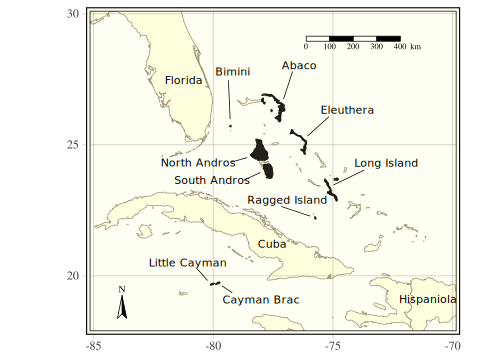
\includegraphics[width=0.8\textwidth]{figures/map.pdf}
	\caption{Map of the West Indies with sampled islands highlighted in black.}
	\label{fig:map}
\end{figure}

% Classification accuracy of SVMs
\begin{figure}[H]
    \centering
	\includegraphics[width=\textwidth]{figures/classif_svm_pca.png}
	\caption{Distributions of classification accuracy across all SVM machines (100 replicates of 5 cross-validation bins each). The dashed line represents the density of a corresponding null binomial distribution, which would be expected under random guessing (testing sets with 20\% of the observations for each island and success probability of $1/3$). Inset plots show the corresponding average confusion matrices and represent the proportion of lizards from each habitat (columns) reassigned in each other habitat (rows), with an interpretation guide in the right panel. P-values indicate deviations of the mean classification accuracy to the expected null binomial distribution. *, P < 0.05}
	\label{fig:classif_svm_pca}
\end{figure}

% Boxplots and analyses of variance
\begin{sidewaysfigure}
    \centering
	\includegraphics[width=18cm]{figures/figure_anova.png}
	\caption{Dewlap coloration varies between habitat-types along different dimensions on different islands. (A) Boxplots show the distribution of the data for the five islands with significant differences in dewlap coloration between habitat (P-values in Fig. \ref{fig:classif_svm_pca}), along the first four principal components. We report the P-values of univariate analyses of variance conducted for each island (see Methods). Horizontal bars indicate \textit{post hoc} significant contrasts at a 0.05 error rate (see Methods). *, P < 0.05. (B) Mapping of the reflectance at various wavelengths onto the principal components. Note that PC1 largely represents brightness.}
	\label{fig:boxplots}
\end{sidewaysfigure}

\pagebreak

\section*{Tables}

\begin{sidewaystable}
	\label{tab:anova}
	\caption{Significance of habitat differences in dewlap coloration, using ANOVA for all islands where significant multivariate differences in dewlap coloration were detected by SVMs. Best fitting model: 1, OLS; 2, GLS. df, degrees of freedom. $\Delta$AICc, difference in AICc between the best fitting model and the OLS-model. AICcw, AICc weight. LRT, likelihood ratio test. Log-lik., log-likelihood. $\chi^2$, likelihood ratio. *, P < 0.05; **, P < 0.01, ***, P < 0.001.}
	\centering
	
\begin{tabular}{llrrrrrrrrrl}
\toprule
nesting & variable & best\_fit & df\_model & AICc & dAICc & AICcw & df\_LRT & loglik & lratio & pvalue & signif\\
\midrule
Abaco & PC1 & 1 & 4 & 710.4 & 0.0 & 0.746 & 2 & -357.0 & 0.14 & 0.9308 & \\
Abaco & PC2 & 1 & 4 & 620.1 & 0.0 & 0.882 & 2 & -310.2 & 31.74 & 0.0000 & ***\\
Abaco & PC3 & 1 & 4 & 517.8 & 0.0 & 0.732 & 2 & -257.2 & 27.37 & 0.0000 & ***\\
Abaco & PC4 & 1 & 4 & 440.6 & 0.0 & 0.596 & 2 & -217.2 & 1.36 & 0.5070 & \\
Bimini & PC1 & 1 & 4 & 561.3 & 0.0 & 0.595 & 2 & -283.1 & 7.40 & 0.0248 & *\\
\addlinespace
Bimini & PC2 & 1 & 4 & 448.1 & 0.0 & 0.656 & 2 & -223.8 & 8.09 & 0.0175 & *\\
Bimini & PC3 & 2 & 6 & 405.3 & -0.2 & 0.529 & 2 & -199.2 & 10.39 & 0.0056 & **\\
Bimini & PC4 & 1 & 4 & 274.2 & 0.0 & 0.854 & 2 & -132.7 & 0.33 & 0.8499 & \\
Cayman Brac & PC1 & 2 & 6 & 402.8 & -4.1 & 0.884 & 2 & -200.9 & 13.81 & 0.0010 & **\\
Cayman Brac & PC2 & 1 & 4 & 332.1 & 0.0 & 0.853 & 2 & -165.9 & 8.41 & 0.0149 & *\\
\addlinespace
Cayman Brac & PC3 & 1 & 4 & 295.8 & 0.0 & 0.800 & 2 & -146.6 & 27.16 & 0.0000 & ***\\
Cayman Brac & PC4 & 1 & 4 & 279.2 & 0.0 & 0.897 & 2 & -137.8 & 5.63 & 0.0600 & \\
Little Cayman & PC1 & 1 & 4 & 367.2 & 0.0 & 0.777 & 2 & -186.0 & 8.18 & 0.0167 & *\\
Little Cayman & PC2 & 2 & 6 & 287.6 & -3.6 & 0.859 & 2 & -140.5 & 29.76 & 0.0000 & ***\\
Little Cayman & PC3 & 1 & 4 & 277.7 & 0.0 & 0.669 & 2 & -138.1 & 21.34 & 0.0000 & ***\\
\addlinespace
Little Cayman & PC4 & 1 & 4 & 226.7 & 0.0 & 0.780 & 2 & -110.7 & 2.85 & 0.2410 & \\
Long Island & PC1 & 2 & 6 & 442.3 & -2.1 & 0.740 & 2 & -221.2 & 2.91 & 0.2331 & \\
Long Island & PC2 & 2 & 6 & 351.4 & -3.1 & 0.823 & 2 & -172.6 & 4.52 & 0.1043 & \\
Long Island & PC3 & 1 & 4 & 322.1 & 0.0 & 0.862 & 2 & -160.0 & 11.24 & 0.0036 & **\\
Long Island & PC4 & 1 & 4 & 195.5 & 0.0 & 0.767 & 2 & -92.9 & 6.46 & 0.0395 & *\\
\bottomrule
\end{tabular}

\end{sidewaystable}





\pagebreak

\bibliographystyle{apalike}
\bibliography{library.bib}
	
\beginsupplement
	
%\section*{Supplementary Figures}

%% Map of each island
\begin{figure}[H]
\centering
	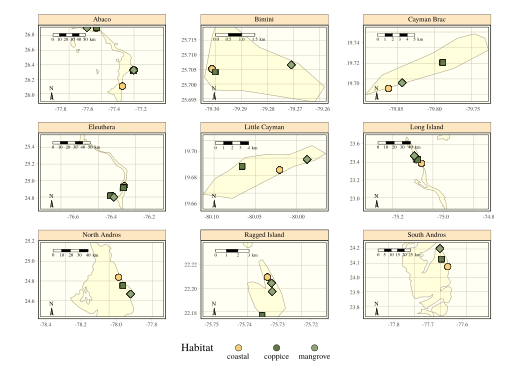
\includegraphics[width=\textwidth]{suppfigures/detailed_map.pdf}
	\caption{Map of the sampling sites and corresponding habitats across nine islands of the West Indies.}
	\label{supfig:map}
\end{figure}

\begin{figure}[H]
	\centering
	\includegraphics[width=0.8\textwidth]{suppfigures/figure_brightness.png}
	\caption{Correlation between dewlap brightness (as measured by the mean reflectance from 300 to 700nm in wavelength) and PC1 score for each island. Pearson's squared correlation coefficients are reported. *, P < 0.05.}	
	\label{supfig:brightness}
\end{figure}

\begin{figure}[H]
	\centering
	\includegraphics[width=0.5\textwidth]{suppfigures/figure_brightness_pooled.png}
	\caption{Correlation between dewlap brightness (as measured by the mean reflectance from 300 to 700nm in wavelength) and PC1 score across the whole archipelago. Pearson's squared correlation coefficient is reported. *, P < 0.05.}
	\label{supfig:brightness_pooled}
\end{figure}

\begin{figure}[H]
	\centering
	\includegraphics[width = \textwidth]{suppfigures/figure_pooled.png}
	\caption{(A) Principal component scores and 5\% confidence ellipses across habitats for the whole archipelago. The principal component analysis was performed on reflectance data from all islands pooled together. (B) PCA rotation matrix showing the loadings of each wavelength from 300 to 700nm onto the principal components.}
	\label{supfig:pooled}
\end{figure}

% Reflectance curves
\begin{figure}[H]
	\centering
	\includegraphics[width=0.8\textwidth]{suppfigures/figure_reflectance.png}
	\caption{5-95th percentile range of lizard dewlap reflectance values (in \% of incoming light) across wavelengths for each island and each habitat.}
	\label{supfig:reflectance}
\end{figure}

\begin{figure}[H]
	\centering
	\includegraphics[width=0.8\textwidth]{suppfigures/classif_svm_pca_pooled.png}
	\caption{Archipelago-wide SVM classification accuracy based on principal component data. Machines were trained on individual dewlaps regardless of island identity. The histogram shows the accuracy distribution over 100 replicates for each five cross-validation bins. The legend is the same as in Figure \ref{fig:classif-svm-pca}.}
	\label{supfig:classif-svm-pca-pooled}
\end{figure}

\begin{figure}[H]
	\centering
	\includegraphics[width=0.8\textwidth]{suppfigures/classif_svm_refl_pooled.png}
	\caption{Archipelago-wide SVM classification accuracy based on reflectance data at 50nm-intervals in wavelength (see Methods). Machines were trained on individual dewlaps regardless of island identity. The histogram shows the accuracy distribution over 100 replicates for each five cross-validation bins. The legend is the same as in Figure \ref{fig:classif-svm-pca}.}
	\label{supfig:classif-svm-refl-pooled}
\end{figure}

\begin{figure}[H]
	\centering
	\includegraphics[width=0.4\textwidth]{suppfigures/importance_svm_pca_pooled.png}
	\caption{Sensitivity analyses of the different input variables in the archipelago-wide SVM classification on principal component data (Figure \ref{supfig:classif-svm-pca-pooled}), with relative importance computed for every machine.}
	\label{supfig:importance-svm-pca-pooled}
\end{figure}

\begin{figure}[H]
	\centering
	\includegraphics[width=0.6\textwidth]{suppfigures/importance_svm_refl_pooled.png}
	\caption{Sensitivity analyses of the different input variables in the archipelago-wide SVM classification on reflectance data at 50nm-intervals in wavelength (Figure \ref{supfig:classif-svm-refl-pooled}), with relative importance computed for every machine.}
	\label{supfig:importance-svm-refl-pooled}
\end{figure}

\begin{figure}[H]
	\centering
	\includegraphics[width=0.8\textwidth]{suppfigures/classif_lda_pca_pooled.png}
	\caption{Archipelago-wide LDA classification accuracy based on principal component data. Machines were trained on individual dewlaps regardless of island identity. The histogram shows the accuracy distribution over 100 replicates for each five cross-validation bins. The legend is the same as in Figure \ref{fig:classif-svm-pca}.}
	\label{supfig:classif-lda-pca-pooled}
\end{figure}

\begin{figure}[H]
	\centering
	\includegraphics[width=0.8\textwidth]{suppfigures/classif_lda_refl_pooled.png}
	\caption{Archipelago-wide LDA classification accuracy based on reflectance data at 50nm-intervals in wavelength (see Methods). Machines were trained on individual dewlaps regardless of island identity. The histogram shows the accuracy distribution over 100 replicates for each five cross-validation bins. The legend is the same as in Figure \ref{fig:classif-svm-pca}.}
	\label{supfig:classif-lda-refl-pooled}
\end{figure}

\begin{figure}[H]
	\centering
	\includegraphics[width=0.5\textwidth]{suppfigures/figure_reflectance_pooled.png}
	\caption{5-95th percentile range of lizard dewlap reflectance values (in \% of incoming light) across wavelengths for each habitat throughout the whole archipelago.}
	\label{supfig:reflectance-pooled}
\end{figure}

\begin{figure}[H]
	\centering
	\includegraphics[width=\textwidth]{suppfigures/classif_lda_pca.png}
	\caption{LDA classification accuracy across islands based on principal component data. Histograms show accuracy distributions over 100 replicates for each five cross-validation bins per island. The legend is the same as in Figure \ref{fig:classif-svm-pca}.}
	\label{supfig:classif-lda-pca}
\end{figure}

\begin{figure}[H]
	\centering
	\includegraphics[width=\textwidth]{suppfigures/classif_svm_refl.png}
	\caption{SVM classification accuracy across islands based on reflectance data at 50nm-intervals in wavelength (see Methods). Histograms show accuracy distributions over 100 replicates for each five cross-validation bins per island. The legend is the same as in Figure \ref{fig:classif-svm-pca}.}
	\label{supfig:classif-svm-refl}
\end{figure}

\begin{figure}[H]
	\centering
	\includegraphics[width=\textwidth]{suppfigures/classif_lda_refl.png}
	\caption{LDA classification accuracy across islands based on reflectance data at 50nm-intervals in wavelength (see Methods). Histograms show accuracy distributions over 100 replicates for each five cross-validation bins per island. The legend is the same as in Figure \ref{fig:classif-svm-pca}.}
	\label{supfig:classif-lda-refl}
\end{figure}

\begin{figure}[H]
	\centering
	\includegraphics[width=0.8\textwidth]{suppfigures/importance_svm_pca.png}
	\caption{Sensitivity analyses of the different input variables in the within-island SVM classification on principal component data (Figure \ref{supfig:classif-svm-pca}), with relative importance computed for every machine.}
	\label{supfig:importance-svm-pca}
\end{figure}

\begin{figure}[H]
	\centering
	\includegraphics[width=0.8\textwidth]{suppfigures/importance_lda_pca.png}
	\caption{Sensitivity analyses of the different input variables in the within-island LDA classification on principal component data (Figure \ref{supfig:classif-lda-pca}), with relative importance computed for every machine.}
	\label{supfig:importance-lda-pca}
\end{figure}

\begin{figure}[H]
	\centering
	\includegraphics[width=0.8\textwidth]{suppfigures/importance_svm_pca.png}
	\caption{Sensitivity analyses of the different input variables in the archipelago-wide SVM classification on reflectance at 50nm-intervals in wavelength (Figure \ref{supfig:classif-svm-refl}), with relative importance computed for every machine.}
	\label{supfig:importance-svm-refl}
\end{figure}

\begin{figure}[H]
	\centering
	\includegraphics[width=0.8\textwidth]{suppfigures/importance_lda_pca.png}
	\caption{Sensitivity analyses of the different input variables in the archipelago-wide LDA classification on reflectance at 50nm-intervals in wavelength (Figure \ref{supfig:classif-lda-refl}), with relative importance computed for every machine.}
	\label{supfig:importance-lda-refl}
\end{figure}

\begin{figure}[H]
	\centering
	\includegraphics[width=\textwidth]{suppfigures/figure_distances2.png}
	\caption{Spatial scale of between-habitat differences in dewlap coloration. For each variable and each pair of habitats where significant differences were detected (Figure \ref{fig:anova}), we performed multiple post hoc pairwise comparisons between the sites involved (Figure \ref{supfig:map}, Table \ref{suptab:sites}), using nonparametric Wilcoxon-Mann-Whitney tests. Here we report, for each pair of habitats, the distances between sites that significantly differed in dewlap coloration at an error rate of 0.05 (P-values corrected with the Benjamini-Hochberg procedure for multiple testing).}
	\label{supfig:distances}
\end{figure}

\begin{figure}[H]
	\centering
	\includegraphics[width=0.7\textwidth]{suppfigures/figure_contrasts.png}
	\caption{Test of parallel divergence between islands. Differences in habitat-means, or contrasts, are shown for two pairs of habitats for each principal component on each island, rescaled so the standard deviation of the means along each principal component is one. The contrasts represent the patterns of between-habtiat variation on each island, for a given principal component. The absence of clustering of islands by variable indicates that islands differ in their between-habitat divergence patterns. This is confirmed by a non-significant MANOVA test of the between versus within-variable variance in contrasts.}
	\label{supfig:contrasts}
\end{figure}

\pagebreak

\section*{Supplementary Figures}

% Map of each island
\begin{figure}[H]
\centering
	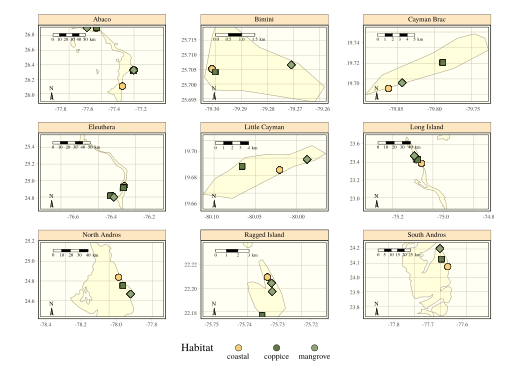
\includegraphics[width=\textwidth]{suppfigures/detailed_map.pdf}
	\caption{Map of the sampling sites and corresponding habitats across nine islands of the West Indies.}
	\label{supfig:map}
\end{figure}

\begin{figure}[H]
	\centering
	\includegraphics[width=0.8\textwidth]{suppfigures/figure_brightness.png}
	\caption{Correlation between dewlap brightness (as measured by the mean reflectance from 300 to 700nm in wavelength) and PC1 score for each island. Pearson's squared correlation coefficients are reported. *, P < 0.05.}	
	\label{supfig:brightness}
\end{figure}

\begin{figure}[H]
	\centering
	\includegraphics[width=0.5\textwidth]{suppfigures/figure_brightness_pooled.png}
	\caption{Correlation between dewlap brightness (as measured by the mean reflectance from 300 to 700nm in wavelength) and PC1 score across the whole archipelago. Pearson's squared correlation coefficient is reported. *, P < 0.05.}
	\label{supfig:brightness_pooled}
\end{figure}

\begin{figure}[H]
	\centering
	\includegraphics[width = \textwidth]{suppfigures/figure_pooled.png}
	\caption{(A) Principal component scores and 5\% confidence ellipses across habitats for the whole archipelago. The principal component analysis was performed on reflectance data from all islands pooled together. (B) PCA rotation matrix showing the loadings of each wavelength from 300 to 700nm onto the principal components.}
	\label{supfig:pooled}
\end{figure}

% Reflectance curves
\begin{figure}[H]
	\centering
	\includegraphics[width=0.8\textwidth]{suppfigures/figure_reflectance.png}
	\caption{5-95th percentile range of lizard dewlap reflectance values (in \% of incoming light) across wavelengths for each island and each habitat.}
	\label{supfig:reflectance}
\end{figure}

\begin{figure}[H]
	\centering
	\includegraphics[width=0.8\textwidth]{suppfigures/classif_svm_pca_pooled.png}
	\caption{Archipelago-wide SVM classification accuracy based on principal component data. Machines were trained on individual dewlaps regardless of island identity. The histogram shows the accuracy distribution over 100 replicates for each five cross-validation bins. The legend is the same as in Figure \ref{fig:classif-svm-pca}.}
	\label{supfig:classif-svm-pca-pooled}
\end{figure}

\begin{figure}[H]
	\centering
	\includegraphics[width=0.8\textwidth]{suppfigures/classif_svm_refl_pooled.png}
	\caption{Archipelago-wide SVM classification accuracy based on reflectance data at 50nm-intervals in wavelength (see Methods). Machines were trained on individual dewlaps regardless of island identity. The histogram shows the accuracy distribution over 100 replicates for each five cross-validation bins. The legend is the same as in Figure \ref{fig:classif-svm-pca}.}
	\label{supfig:classif-svm-refl-pooled}
\end{figure}

\begin{figure}[H]
	\centering
	\includegraphics[width=0.4\textwidth]{suppfigures/importance_svm_pca_pooled.png}
	\caption{Sensitivity analyses of the different input variables in the archipelago-wide SVM classification on principal component data (Figure \ref{supfig:classif-svm-pca-pooled}), with relative importance computed for every machine.}
	\label{supfig:importance-svm-pca-pooled}
\end{figure}

\begin{figure}[H]
	\centering
	\includegraphics[width=0.6\textwidth]{suppfigures/importance_svm_refl_pooled.png}
	\caption{Sensitivity analyses of the different input variables in the archipelago-wide SVM classification on reflectance data at 50nm-intervals in wavelength (Figure \ref{supfig:classif-svm-refl-pooled}), with relative importance computed for every machine.}
	\label{supfig:importance-svm-refl-pooled}
\end{figure}

\begin{figure}[H]
	\centering
	\includegraphics[width=0.8\textwidth]{suppfigures/classif_lda_pca_pooled.png}
	\caption{Archipelago-wide LDA classification accuracy based on principal component data. Machines were trained on individual dewlaps regardless of island identity. The histogram shows the accuracy distribution over 100 replicates for each five cross-validation bins. The legend is the same as in Figure \ref{fig:classif-svm-pca}.}
	\label{supfig:classif-lda-pca-pooled}
\end{figure}

\begin{figure}[H]
	\centering
	\includegraphics[width=0.8\textwidth]{suppfigures/classif_lda_refl_pooled.png}
	\caption{Archipelago-wide LDA classification accuracy based on reflectance data at 50nm-intervals in wavelength (see Methods). Machines were trained on individual dewlaps regardless of island identity. The histogram shows the accuracy distribution over 100 replicates for each five cross-validation bins. The legend is the same as in Figure \ref{fig:classif-svm-pca}.}
	\label{supfig:classif-lda-refl-pooled}
\end{figure}

\begin{figure}[H]
	\centering
	\includegraphics[width=0.5\textwidth]{suppfigures/figure_reflectance_pooled.png}
	\caption{5-95th percentile range of lizard dewlap reflectance values (in \% of incoming light) across wavelengths for each habitat throughout the whole archipelago.}
	\label{supfig:reflectance-pooled}
\end{figure}

\begin{figure}[H]
	\centering
	\includegraphics[width=\textwidth]{suppfigures/classif_lda_pca.png}
	\caption{LDA classification accuracy across islands based on principal component data. Histograms show accuracy distributions over 100 replicates for each five cross-validation bins per island. The legend is the same as in Figure \ref{fig:classif-svm-pca}.}
	\label{supfig:classif-lda-pca}
\end{figure}

\begin{figure}[H]
	\centering
	\includegraphics[width=\textwidth]{suppfigures/classif_svm_refl.png}
	\caption{SVM classification accuracy across islands based on reflectance data at 50nm-intervals in wavelength (see Methods). Histograms show accuracy distributions over 100 replicates for each five cross-validation bins per island. The legend is the same as in Figure \ref{fig:classif-svm-pca}.}
	\label{supfig:classif-svm-refl}
\end{figure}

\begin{figure}[H]
	\centering
	\includegraphics[width=\textwidth]{suppfigures/classif_lda_refl.png}
	\caption{LDA classification accuracy across islands based on reflectance data at 50nm-intervals in wavelength (see Methods). Histograms show accuracy distributions over 100 replicates for each five cross-validation bins per island. The legend is the same as in Figure \ref{fig:classif-svm-pca}.}
	\label{supfig:classif-lda-refl}
\end{figure}

\begin{figure}[H]
	\centering
	\includegraphics[width=0.8\textwidth]{suppfigures/importance_svm_pca.png}
	\caption{Sensitivity analyses of the different input variables in the within-island SVM classification on principal component data (Figure \ref{supfig:classif-svm-pca}), with relative importance computed for every machine.}
	\label{supfig:importance-svm-pca}
\end{figure}

\begin{figure}[H]
	\centering
	\includegraphics[width=0.8\textwidth]{suppfigures/importance_lda_pca.png}
	\caption{Sensitivity analyses of the different input variables in the within-island LDA classification on principal component data (Figure \ref{supfig:classif-lda-pca}), with relative importance computed for every machine.}
	\label{supfig:importance-lda-pca}
\end{figure}

\begin{figure}[H]
	\centering
	\includegraphics[width=0.8\textwidth]{suppfigures/importance_svm_pca.png}
	\caption{Sensitivity analyses of the different input variables in the archipelago-wide SVM classification on reflectance at 50nm-intervals in wavelength (Figure \ref{supfig:classif-svm-refl}), with relative importance computed for every machine.}
	\label{supfig:importance-svm-refl}
\end{figure}

\begin{figure}[H]
	\centering
	\includegraphics[width=0.8\textwidth]{suppfigures/importance_lda_pca.png}
	\caption{Sensitivity analyses of the different input variables in the archipelago-wide LDA classification on reflectance at 50nm-intervals in wavelength (Figure \ref{supfig:classif-lda-refl}), with relative importance computed for every machine.}
	\label{supfig:importance-lda-refl}
\end{figure}

\begin{figure}[H]
	\centering
	\includegraphics[width=\textwidth]{suppfigures/figure_distances2.png}
	\caption{Spatial scale of between-habitat differences in dewlap coloration. For each variable and each pair of habitats where significant differences were detected (Figure \ref{fig:anova}), we performed multiple post hoc pairwise comparisons between the sites involved (Figure \ref{supfig:map}, Table \ref{suptab:sites}), using nonparametric Wilcoxon-Mann-Whitney tests. Here we report, for each pair of habitats, the distances between sites that significantly differed in dewlap coloration at an error rate of 0.05 (P-values corrected with the Benjamini-Hochberg procedure for multiple testing).}
	\label{supfig:distances}
\end{figure}

\begin{figure}[H]
	\centering
	\includegraphics[width=0.7\textwidth]{suppfigures/figure_contrasts.png}
	\caption{Test of parallel divergence between islands. Differences in habitat-means, or contrasts, are shown for two pairs of habitats for each principal component on each island, rescaled so the standard deviation of the means along each principal component is one. The contrasts represent the patterns of between-habtiat variation on each island, for a given principal component. The absence of clustering of islands by variable indicates that islands differ in their between-habitat divergence patterns. This is confirmed by a non-significant MANOVA test of the between versus within-variable variance in contrasts.}
	\label{supfig:contrasts}
\end{figure}

\pagebreak

\section*{Supplementary Tables}

\begin{table}
	\label{suptab:counts}	
	\caption{Number of lizards sampled in each habitat on each island.}
	\centering
	% Sample sizes
\begin{table}[H]
    \caption{Numbers of lizards sampled across islands and habitats.}
    \centering
    \begin{tabular}{lrrr}
        \hline
        & coastal & coppice & mangrove\\
        \hline
        Abaco & 41 & 24 & 21\\
        Bimini & 38 & 14 & 15\\
        Cayman Brac & 15 & 18 & 17\\
        Eleuthera & 22 & 25 & 9\\
        Little Cayman & 17 & 12 & 16\\
        Long Island & 26 & 14 & 13\\
        North Andros & 9 & 9 & 10\\
        Ragged Island & 18 & 15 & 17\\
        South Andros & 10 & 9 & 12\\
        \hline
    \end{tabular}
    \label{suptab:counts}
\end{table}
\end{table}

\begin{table}
	\label{suptab:sites}
	\caption{Locations of the sampling sites across islands, with mean principal component scores per site.}
	\centering
	
\begin{tabular}{lrrlrrrr}
\toprule
Island & Longitude & Latitude & Habitat & PC1 & PC2 & PC3 & PC4\\
\midrule
Abaco & -77.7256 & 26.9083 & mangrove & -5.4905 & 1.3541 & -0.4741 & 0.0083\\
Abaco & -77.5800 & 26.9020 & coastal & 1.8633 & 0.0365 & -0.4475 & 0.0033\\
Abaco & -77.5763 & 26.9128 & coppice & -1.6738 & -1.7793 & -0.0499 & 0.0012\\
Abaco & -77.1784 & 26.1045 & coastal & 1.1863 & 2.0408 & -0.3468 & 0.0022\\
Abaco & -77.0055 & 26.3254 & mangrove & -9.0319 & -2.7460 & 0.4687 & 0.0077\\
Abaco & -77.0039 & 26.3170 & coppice & 0.9967 & 0.5161 & -0.0267 & -0.0118\\
Abaco & -76.9968 & 26.3260 & coastal & 7.6077 & 0.3186 & 0.1771 & -0.0008\\
Bimini & -79.3022 & 25.5859 & coastal & 5.7537 & -0.1593 & -0.2505 & 0.0001\\
Bimini & -79.3014 & 25.7052 & coastal & -3.1822 & 1.6617 & -0.0460 & 0.0024\\
Bimini & -79.3002 & 25.7042 & coppice & -1.3514 & -3.8786 & 0.1027 & -0.0027\\
Bimini & -79.2709 & 25.7066 & mangrove & 3.3656 & 0.6244 & 0.1569 & -0.0021\\
Cayman Brac & -79.8627 & 19.6878 & coastal & 6.6606 & -2.5670 & 0.0166 & -0.0007\\
Cayman Brac & -79.8441 & 19.6949 & mangrove & -1.0914 & 4.3607 & 0.0855 & 0.0001\\
Cayman Brac & -79.7887 & 19.7209 & coppice & -4.5197 & -1.9793 & -0.0946 & 0.0004\\
Eleuthera & -76.3347 & 24.8146 & coppice & 3.2669 & -1.2404 & 0.1018 & -0.0085\\
Eleuthera & -76.3058 & 24.8127 & coastal & 0.4216 & -3.5133 & -0.0567 & 0.0009\\
Eleuthera & -76.2901 & 24.7981 & mangrove & 2.1881 & 0.7517 & 0.3957 & -0.0055\\
Eleuthera & -76.1616 & 24.9129 & coppice & -1.9136 & 1.0868 & -0.4978 & -0.0092\\
Eleuthera & -76.1492 & 24.9335 & coastal & -3.1863 & 2.4270 & 0.1881 & 0.0218\\
Little Cayman & -80.0660 & 19.6906 & coppice & 0.8021 & -1.9569 & -0.0760 & -0.0068\\
Little Cayman & -80.0205 & 19.6865 & coastal & -6.6917 & -1.2615 & 0.0659 & 0.0057\\
Little Cayman & -79.9871 & 19.6986 & mangrove & 6.5083 & 2.8079 & -0.0129 & -0.0010\\
Long Island & -75.2299 & 23.4740 & mangrove & -1.2873 & 1.9371 & -0.1880 & -0.0029\\
Long Island & -75.2063 & 23.4282 & coastal & 2.3686 & -0.9033 & 0.0215 & 0.0096\\
Long Island & -75.1884 & 23.4292 & coppice & -4.6266 & 0.5060 & 0.1049 & -0.0070\\
Long Island & -75.1408 & 23.3883 & coastal & 3.6139 & -1.4521 & 0.0475 & 0.0025\\
North Andros & -77.8908 & 24.8391 & coastal & -2.1881 & -1.1236 & 0.0397 & -0.0060\\
North Andros & -77.8428 & 24.7516 & coppice & -1.8115 & 0.0012 & -0.1678 & 0.0024\\
North Andros & -77.7540 & 24.6644 & mangrove & 3.5997 & 1.0101 & 0.1153 & 0.0033\\
Ragged Island & -75.7364 & 22.1768 & coppice & 3.2851 & -0.3274 & 0.1911 & -0.0013\\
Ragged Island & -75.7314 & 22.2097 & coastal & -0.6412 & -0.8878 & -0.1293 & -0.0033\\
Ragged Island & -75.7276 & 22.2045 & mangrove & -2.9188 & 1.5792 & -0.0034 & 0.0099\\
Ragged Island & -75.7270 & 22.1973 & mangrove & -1.2210 & 0.7285 & -0.0721 & -0.0028\\
South Andros & -77.6050 & 24.2027 & mangrove & -3.9253 & 0.4734 & 0.0477 & -0.0005\\
South Andros & -77.5936 & 24.1289 & coppice & 6.1152 & -0.4925 & 0.0349 & 0.0012\\
South Andros & -77.5453 & 24.0764 & coastal & -0.7933 & -0.1248 & -0.0887 & -0.0004\\
\bottomrule
\end{tabular}

\end{table}

\begin{table}
	\label{suptab:pcavariances}
	\caption{Proportion of variance explained by the first four principal components on each island, as well as across the whole archipelago.}
	\centering
	
\begin{tabular}{l|r|r|r|r|r}
\hline
island & PC1 & PC2 & PC3 & PC4 & total\\
\hline
Abaco & 0.400 & 0.279 & 0.147 & 0.079 & 0.906\\
\hline
Bimini & 0.502 & 0.208 & 0.160 & 0.051 & 0.921\\
\hline
Cayman Brac & 0.438 & 0.190 & 0.155 & 0.105 & 0.888\\
\hline
Eleuthera & 0.490 & 0.233 & 0.138 & 0.066 & 0.926\\
\hline
Little Cayman & 0.441 & 0.212 & 0.176 & 0.078 & 0.907\\
\hline
Long Island & 0.515 & 0.205 & 0.161 & 0.043 & 0.925\\
\hline
North Andros & 0.560 & 0.170 & 0.152 & 0.054 & 0.937\\
\hline
Ragged Island & 0.483 & 0.226 & 0.127 & 0.072 & 0.907\\
\hline
South Andros & 0.488 & 0.247 & 0.146 & 0.067 & 0.948\\
\hline
Archipelago & 0.473 & 0.197 & 0.164 & 0.079 & 0.913\\
\hline
\end{tabular}

\end{table}

\begin{table}
	\label{suptab:brightness}
	\caption{Pearson's correlation test between dewlap brightness, as measured by the average reflectance between 300 and 700nm in wavelength, and PC1 scores, for all islands and across the whole archipelago. ***, P < 0.001.}
	\centering
	
\begin{tabular}{l|r|l|l}
\hline
island & r2 & pvalue & \\
\hline
Abaco & 0.908 & < 0.0001 & ***\\
\hline
Bimini & 0.999 & < 0.0001 & ***\\
\hline
Cayman Brac & 0.987 & < 0.0001 & ***\\
\hline
Eleuthera & 0.963 & < 0.0001 & ***\\
\hline
Little Cayman & 0.965 & < 0.0001 & ***\\
\hline
Long Island & 0.986 & < 0.0001 & ***\\
\hline
North Andros & 0.994 & < 0.0001 & ***\\
\hline
Ragged Island & 0.978 & < 0.0001 & ***\\
\hline
South Andros & 0.979 & < 0.0001 & ***\\
\hline
Archipelago & 0.976 & < 0.0001 & ***\\
\hline
\end{tabular}

\end{table}

\begin{table}
	\label{suptab:multinorm}
	\caption{Henze-Zirkler's test of multivariate normality, performed on principal components in each habitat and on each island. HZ, test statistic. *, P < 0.05; **, P < 0.01; ***, P < 0.001.}
	\centering
	
\begin{tabular}{llrrl}
\toprule
island & habitat & HZ & pvalue & signif\\
\midrule
Abaco & coastal & 1.10 & 0.0027 & **\\
Abaco & coppice & 1.07 & 0.0022 & **\\
Abaco & mangrove & 1.06 & 0.0023 & **\\
Bimini & coastal & 1.28 & 0.0001 & ***\\
Bimini & coppice & 0.85 & 0.0482 & *\\
\addlinespace
Bimini & mangrove & 1.19 & 0.0001 & ***\\
Cayman Brac & coastal & 0.65 & 0.5311 & \\
Cayman Brac & coppice & 0.70 & 0.3940 & \\
Cayman Brac & mangrove & 0.66 & 0.5357 & \\
Eleuthera & coastal & 1.61 & 0.0000 & ***\\
\addlinespace
Eleuthera & coppice & 1.48 & 0.0000 & ***\\
Eleuthera & mangrove & 0.73 & 0.1423 & \\
Little Cayman & coastal & 0.62 & 0.6599 & \\
Little Cayman & coppice & 0.64 & 0.4867 & \\
Little Cayman & mangrove & 0.87 & 0.0413 & *\\
\addlinespace
Long Island & coastal & 0.82 & 0.1468 & \\
Long Island & coppice & 0.92 & 0.0150 & *\\
Long Island & mangrove & 0.77 & 0.1289 & \\
North Andros & coastal & 0.66 & 0.3174 & \\
North Andros & coppice & 0.76 & 0.0900 & \\
\addlinespace
North Andros & mangrove & 0.67 & 0.3185 & \\
Ragged Island & coastal & 0.76 & 0.2268 & \\
Ragged Island & coppice & 0.80 & 0.1115 & \\
Ragged Island & mangrove & 0.54 & 0.9022 & \\
South Andros & coastal & 0.66 & 0.3451 & \\
\addlinespace
South Andros & coppice & 0.66 & 0.3154 & \\
South Andros & mangrove & 0.91 & 0.0144 & *\\
\bottomrule
\end{tabular}

\end{table}

\begin{table}
	\label{suptab:covariance}
	\caption{Box's M-test of homogeneity of covariance matrices across habitats on each island. $\chi^2$, test statistic. *, P < 0.05; **, P < 0.01; ***, P < 0.001.}
	\centering
	
\begin{tabular}{lrrrl}
\toprule
island & chisq & df & pvalue & signif\\
\midrule
Abaco & 47.1 & 20 & 0.0006 & ***\\
Bimini & 36.0 & 20 & 0.0152 & *\\
Cayman Brac & 36.9 & 20 & 0.0120 & *\\
Eleuthera & 44.6 & 20 & 0.0013 & **\\
Little Cayman & 32.8 & 20 & 0.0356 & *\\
\addlinespace
Long Island & 56.2 & 20 & 0.0000 & ***\\
North Andros & 33.7 & 20 & 0.0283 & *\\
Ragged Island & 29.3 & 20 & 0.0824 & \\
South Andros & 46.5 & 20 & 0.0007 & ***\\
\bottomrule
\end{tabular}

\end{table}

\begin{table}
	\label{suptab:normality}
	\caption{Shapiro-Wilk's test of univariate normality performed on each island where significant differences were detected by SVM classification, in each habitat where deviations from multivariate normality were detected. $W$, test statistic. *, P < 0.05; **, P < 0.01; ***, P < 0.001.}
	\centering
	
\begin{tabular}{lllrrl}
\toprule
island & habitat & variable & W & pvalue & signif\\
\midrule
Abaco & coastal & PC1 & 0.954 & 0.0941 & \\
Abaco & coastal & PC2 & 0.927 & 0.0112 & *\\
Abaco & coastal & PC3 & 0.973 & 0.4228 & \\
Abaco & coastal & PC4 & 0.955 & 0.1027 & \\
Abaco & coppice & PC1 & 0.970 & 0.6776 & \\
\addlinespace
Abaco & coppice & PC2 & 0.816 & 0.0005 & ***\\
Abaco & coppice & PC3 & 0.930 & 0.0976 & \\
Abaco & coppice & PC4 & 0.941 & 0.1711 & \\
Abaco & mangrove & PC1 & 0.881 & 0.0155 & *\\
Abaco & mangrove & PC2 & 0.869 & 0.0093 & **\\
\addlinespace
Abaco & mangrove & PC3 & 0.986 & 0.9873 & \\
Abaco & mangrove & PC4 & 0.939 & 0.2044 & \\
Bimini & coastal & PC1 & 0.821 & 0.0000 & ***\\
Bimini & coastal & PC2 & 0.960 & 0.1854 & \\
Bimini & coastal & PC3 & 0.856 & 0.0002 & ***\\
\addlinespace
Bimini & coastal & PC4 & 0.945 & 0.0611 & \\
Bimini & coppice & PC1 & 0.911 & 0.1648 & \\
Bimini & coppice & PC2 & 0.958 & 0.6927 & \\
Bimini & coppice & PC3 & 0.953 & 0.6146 & \\
Bimini & coppice & PC4 & 0.971 & 0.8953 & \\
\addlinespace
Bimini & mangrove & PC1 & 0.884 & 0.0536 & \\
Bimini & mangrove & PC2 & 0.976 & 0.9363 & \\
Bimini & mangrove & PC3 & 0.982 & 0.9805 & \\
Bimini & mangrove & PC4 & 0.975 & 0.9232 & \\
Eleuthera & coastal & PC1 & 0.909 & 0.0461 & *\\
\addlinespace
Eleuthera & coastal & PC2 & 0.886 & 0.0157 & *\\
Eleuthera & coastal & PC3 & 0.906 & 0.0390 & *\\
Eleuthera & coastal & PC4 & 0.962 & 0.5293 & \\
Eleuthera & coppice & PC1 & 0.922 & 0.0567 & \\
Eleuthera & coppice & PC2 & 0.954 & 0.3055 & \\
\addlinespace
Eleuthera & coppice & PC3 & 0.781 & 0.0001 & ***\\
Eleuthera & coppice & PC4 & 0.901 & 0.0188 & *\\
Little Cayman & mangrove & PC1 & 0.907 & 0.1024 & \\
Little Cayman & mangrove & PC2 & 0.904 & 0.0924 & \\
Little Cayman & mangrove & PC3 & 0.739 & 0.0005 & ***\\
\addlinespace
Little Cayman & mangrove & PC4 & 0.973 & 0.8802 & \\
Long Island & coppice & PC1 & 0.686 & 0.0003 & ***\\
Long Island & coppice & PC2 & 0.848 & 0.0210 & *\\
Long Island & coppice & PC3 & 0.931 & 0.3188 & \\
Long Island & coppice & PC4 & 0.904 & 0.1280 & \\
\addlinespace
South Andros & mangrove & PC1 & 0.787 & 0.0067 & **\\
South Andros & mangrove & PC2 & 0.861 & 0.0500 & *\\
South Andros & mangrove & PC3 & 0.697 & 0.0008 & ***\\
South Andros & mangrove & PC4 & 0.950 & 0.6411 & \\
\bottomrule
\end{tabular}

\end{table}

\begin{table}
	\label{suptab:anova-pooled}
	\caption{Univariate ANOVAs performed on each principal component across the whole archipelago. Legend is the same as for Table \ref{tab:anova}, except that best fitting models 3 and 4 refer to the mixed effect equivalents to the OLS and GLS model, with island as a random effect (see Methods).}
	\centering
	
\begin{tabular}{lrrrrrrrrrl}
\toprule
variable & best\_fit & df\_model & AICc & dAICc & AICcw & df\_LRT & loglik & lratio & pvalue & signif\\
\midrule
PC1 & 3 & 5 & 3749.9 & -228.3 & 0.613 & 2 & -1874.7 & 8.69 & 0.0130 & *\\
PC2 & 4 & 7 & 3002.2 & -162.3 & 0.976 & 2 & -1496.2 & 17.76 & 0.0001 & ***\\
PC3 & 4 & 7 & 2826.3 & -175.4 & 0.968 & 2 & -1407.8 & 7.03 & 0.0298 & *\\
PC4 & 4 & 7 & 2015.7 & -305.8 & 0.519 & 2 & -1000.1 & 0.47 & 0.7914 & \\
\bottomrule
\end{tabular}

\end{table}

\begin{table}
	\label{suptab:classif-svm-pca}
	\caption{Mean SVM classification accuracy per island, over all replicates and cross-validation bins. $N$, number of observations per island; $p_{\mbox{test}}$, proportion of the data sampled to form the training set; $n_{\mbox{test}}$, number of observations in the testing set. P-values indicate deviations from the expected null binomial distribution, with $n_{\mbox{test}}$ events per island and random guess success probability $1/3$. *, P < 0.05, **, P < 0.01, ***, P < 0.001.}
	\centering
	
\begin{tabular}{lrrrrrl}
\toprule
Island & Accuracy & N & $p_{\mbox{test}}$ & $n_{\mbox{test}}$ & $P$ & \\
\midrule
Abaco & 0.612 & 86 & 0.2 & 17 & 0.0080 & **\\
Bimini & 0.547 & 67 & 0.2 & 13 & 0.0347 & *\\
Cayman Brac & 0.721 & 50 & 0.2 & 10 & 0.0034 & **\\
Eleuthera & 0.437 & 56 & 0.2 & 11 & 0.2890 & \\
Little Cayman & 0.734 & 45 & 0.2 & 9 & 0.0083 & **\\
Long Island & 0.651 & 53 & 0.2 & 10 & 0.0197 & *\\
North Andros & 0.453 & 28 & 0.2 & 5 & 0.2099 & \\
Ragged Island & 0.364 & 50 & 0.2 & 10 & 0.4407 & \\
South Andros & 0.600 & 31 & 0.2 & 6 & 0.1001 & \\
\bottomrule
\end{tabular}

\end{table}

\begin{table}
	\label{suptab:kruskal}
	\caption{Results of nonparametric Kruskal-Wallis tests performed on each variable on each island where deviations from normality were detected.}
	\centering
	
\begin{tabular}{llrrrl}
\toprule
Island & Variable & $\chi^2$ & df & $P$ & \\
\midrule
Abaco & PC1 & 0.74 & 2 & 0.6924 & \\
Abaco & PC2 & 23.13 & 2 & 0.0000 & ***\\
Bimini & PC1 & 7.38 & 2 & 0.0250 & *\\
Bimini & PC3 & 15.17 & 2 & 0.0005 & ***\\
Little Cayman & PC3 & 19.95 & 2 & 0.0000 & ***\\
Long Island & PC1 & 10.98 & 2 & 0.0041 & **\\
Long Island & PC2 & 4.02 & 2 & 0.1339 & \\
\bottomrule
\end{tabular}

\end{table}

\begin{table}
	\label{suptab:autocor}
	\caption{Individual-based permutation tests of spatial autocorrelation within islands. P-values were computed from 1,000 permutations of individual site-labels. Pearson's coefficient $r$ measures the correlation between distances in color space and geodesic distances among the sites. $N$, number of sites. *, P < 0.05.}
	\centering
	
\begin{tabular}{lrrrl}
\toprule
Island & $r^2$ & $P$ & N & \\
\midrule
Abaco & -0.213 & 0.817 & 7 & \\
Bimini & 0.044 & 0.510 & 4 & \\
Cayman Brac & -0.010 & 0.465 & 3 & \\
Eleuthera & 0.816 & 0.015 & 5 & *\\
Little Cayman & -0.688 & 0.684 & 3 & \\
Long Island & -0.189 & 0.579 & 4 & \\
North Andros & 0.730 & 0.199 & 3 & \\
Ragged Island & 0.706 & 0.114 & 4 & \\
South Andros & -0.852 & 0.776 & 3 & \\
\bottomrule
\end{tabular}

\end{table}

\end{document}

